\begin{figure}[!t]
\centering
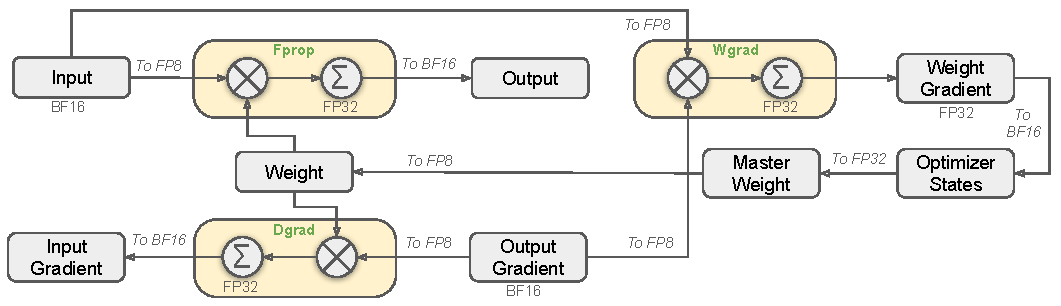
\includegraphics[width=0.99\linewidth]{figures/fp8-frameworkv3.pdf}
\caption{
    The overall mixed precision framework with FP8 data format. For clarification, only the \texttt{Linear} operator is illustrated. 
}
\label{fig:fp8_framework}
\end{figure}

Inspired by recent advances in low-precision training~\citep{fp8lm, llm.int8, 8-bit-numerical}, we propose a fine-grained mixed precision framework utilizing the FP8 data format for training \dsviii{}. 
While low-precision training holds great promise, it is often limited by the presence of outliers in activations, weights, and gradients~\citep{massiveoutlier, understandoutlier, scalefp8train}. 
Although significant progress has been made in inference quantization~\citep{xiao2023smoothquant, frantar2022gptq}, there are relatively few studies demonstrating successful application of low-precision techniques in large-scale language model pre-training~\citep{scalefp8train}. 
To address this challenge and effectively extend the dynamic range of the FP8 format, we introduce a fine-grained quantization strategy: tile-wise grouping with $1\times N_c$ elements or block-wise grouping with $N_c\times N_c$ elements. 
The associated dequantization overhead is largely mitigated under our increased-precision accumulation process, a critical aspect for achieving accurate FP8 General Matrix Multiplication~(GEMM). 
Moreover, to further reduce memory and communication overhead in MoE training, we cache and dispatch activations in FP8, while storing low-precision optimizer states in BF16. 
We validate the proposed FP8 mixed precision framework on two model scales similar to \dsvii{}-Lite and \dsvii{}, training for approximately 1 trillion tokens (see more details in Appendix~\ref{app:fp8_cp_bf16}). 
Notably, compared with the BF16 baseline, the relative loss error of our FP8-training model remains consistently below 0.25\%, a level well within the acceptable range of training randomness.

\subsubsection{Mixed Precision Framework}
Building upon widely adopted techniques in low-precision training~\citep{bf16train, fp16train}, we propose a mixed precision framework for FP8 training. 
In this framework, most compute-density operations are conducted in FP8, while a few key operations are strategically maintained in their original data formats to balance training efficiency and numerical stability. 
The overall framework is illustrated in Figure~\ref{fig:fp8_framework}.

Firstly, in order to accelerate model training, the majority of core computation kernels, i.e., GEMM operations, are implemented in FP8 precision. 
These GEMM operations accept FP8 tensors as inputs and produce outputs in BF16 or FP32. 
As depicted in Figure~\ref{fig:fp8_framework}, all three GEMMs associated with the \texttt{Linear} operator, namely \texttt{Fprop} (forward pass), \texttt{Dgrad} (activation backward pass), and \texttt{Wgrad} (weight backward pass), are executed in FP8. 
This design theoretically doubles the computational speed compared with the original BF16 method. 
Additionally, the FP8 \texttt{Wgrad} GEMM allows activations to be stored in FP8 for use in the backward pass. 
This significantly reduces memory consumption.

Despite the efficiency advantage of the FP8 format, certain operators still require a higher precision due to their sensitivity to low-precision computations. 
Besides, some low-cost operators can also utilize a higher precision with a negligible overhead to the overall training cost. 
For this reason, after careful investigations, we maintain the original precision (e.g., BF16 or FP32) for the following components: the embedding module, the output head, MoE gating modules, normalization operators, and attention operators. 
These targeted retentions of high precision ensure stable training dynamics for \dsviii{}.
To further guarantee numerical stability, we store the master weights, weight gradients, and optimizer states in higher precision. 
While these high-precision components incur some memory overheads, their impact can be minimized through efficient sharding across multiple DP ranks in our distributed training system.

\begin{figure}[!t]
\centering
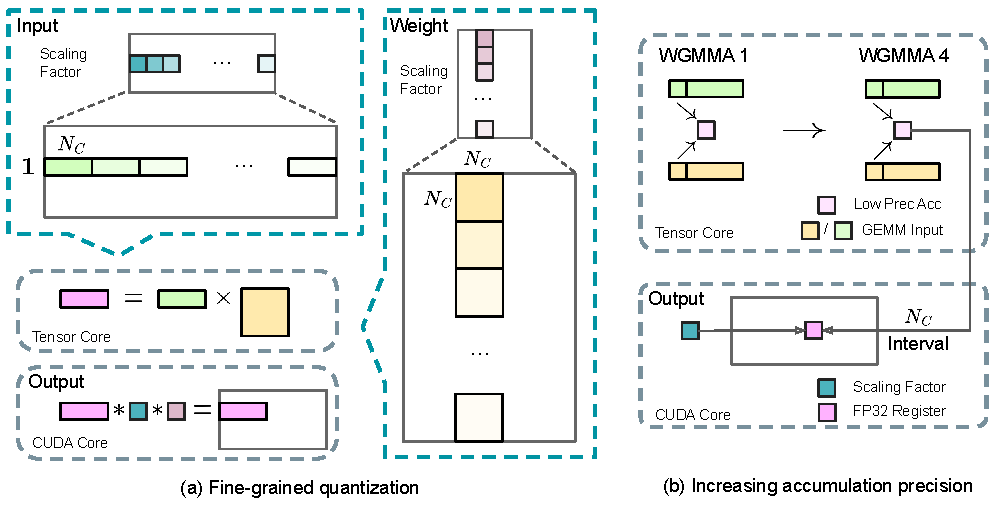
\includegraphics[width=0.95\linewidth]{figures/fp8-128accumulatorv4.pdf}
\caption{
    (a) We propose a fine-grained quantization method to mitigate quantization errors caused by feature outliers; for illustration simplicity, only \texttt{Fprop} is illustrated. 
    (b) In conjunction with our quantization strategy, we improve the FP8 GEMM precision by promoting to CUDA Cores at an interval of $N_C=128$ elements MMA for the high-precision accumulation. 
}
\label{fig:fp8_quantization}
\end{figure}

\subsubsection{Improved Precision from Quantization and Multiplication}
Based on our mixed precision FP8 framework, we introduce several strategies to enhance low-precision training accuracy, focusing on both the quantization method and the multiplication process.

\paragraph{Fine-Grained Quantization.}
In low-precision training frameworks, overflows and underflows are common challenges due to the limited dynamic range of the FP8 format, which is constrained by its reduced exponent bits. 
As a standard practice, the input distribution is aligned to the representable range of the FP8 format by scaling the maximum absolute value of the input tensor to the maximum representable value of FP8~\citep{fp16train}. 
This method makes low-precision training highly sensitive to activation outliers, which can heavily degrade quantization accuracy.
To solve this, we propose a fine-grained quantization method that applies scaling at a more granular level. 
As illustrated in Figure~\ref{fig:fp8_quantization} (a), (1) for activations, we group and scale elements on a \texttt{1x128} tile basis (i.e., per token per 128 channels); and (2) for weights, we group and scale elements on a \texttt{128x128} block basis (i.e., per 128 input channels per 128 output channels).
This approach ensures that the quantization process can better accommodate outliers by adapting the scale according to smaller groups of elements. 
In Appendix~\ref{app:fp8_blockwise}, we further discuss the training instability when we group and scale activations on a block basis in the same way as weights quantization.

One key modification in our method is the introduction of per-group scaling factors along the inner dimension of GEMM operations. 
This functionality is not directly supported in the standard FP8 GEMM. 
However, combined with our precise FP32 accumulation strategy, it can be efficiently implemented. 
% We will elaborate it in the following paragraph.

Notably, our fine-grained quantization strategy is highly consistent with the idea of microscaling formats~\citep{rouhani2023microscaling}, while the Tensor Cores of NVIDIA next-generation GPUs (Blackwell series) have announced the support for microscaling formats with smaller quantization granularity~\citep{nvidia_tensor_cores}. 
We hope our design can serve as a reference for future work to keep pace with the latest GPU architectures.

\paragraph{Increasing Accumulation Precision.}
Low-precision GEMM operations often suffer from underflow issues, and their accuracy largely depends on high-precision accumulation, which is commonly performed in an FP32 precision~\citep{bf16train, fp16train}.
However, we observe that the accumulation precision of FP8 GEMM on NVIDIA H800 GPUs is limited to retaining around 14 bits, which is significantly lower than FP32 accumulation precision. 
This problem will become more pronounced when the inner dimension \texttt{K} is large~\citep{switchback}, a typical scenario in large-scale model training where the batch size and model width are increased. 
Taking GEMM operations of two random matrices with \texttt{K} = 4096 for example, in our preliminary test, the limited accumulation precision in Tensor Cores results in a maximum relative error of nearly 2\%. 
Despite these problems, the limited accumulation precision is still the default option in a few FP8 frameworks~\citep{transformerengine}, severely constraining the training accuracy. 

In order to address this issue, we adopt the strategy of promotion to CUDA Cores for higher precision~\citep{Thakkar_CUTLASS_2023}. 
The process is illustrated in Figure~\ref{fig:fp8_quantization} (b). 
To be specific, during MMA (Matrix Multiply-Accumulate) execution on Tensor Cores, intermediate results are accumulated using the limited bit width. 
Once an interval of $N_C$ is reached, these partial results will be copied to FP32 registers on CUDA Cores, where full-precision FP32 accumulation is performed.
As mentioned before, our fine-grained quantization applies per-group scaling factors along the inner dimension \texttt{K}. 
These scaling factors can be efficiently multiplied on the CUDA Cores as the dequantization process with minimal additional computational cost.

It is worth noting that this modification reduces the WGMMA (Warpgroup-level Matrix Multiply-Accumulate) instruction issue rate for a single warpgroup. However, on the H800 architecture, it is typical for two WGMMA to persist concurrently: while one warpgroup performs the promotion operation, the other is able to execute the MMA operation. This design enables overlapping of the two operations, maintaining high utilization of Tensor Cores.
Based on our experiments, setting $N_C=128$ elements, equivalent to 4 WGMMAs, represents the minimal accumulation interval that can significantly improve precision without introducing substantial overhead.

\paragraph{Mantissa over Exponents.} 
In contrast to the hybrid FP8 format adopted by prior work \citep{transformerengine, fp8lm, hfp8}, which uses \texttt{E4M3} (4-bit exponent and 3-bit mantissa) in \texttt{Fprop} and \texttt{E5M2} (5-bit exponent and 2-bit mantissa) in \texttt{Dgrad} and \texttt{Wgrad}, we adopt the \texttt{E4M3} format on all tensors for higher precision. 
We attribute the feasibility of this approach to our fine-grained quantization strategy, i.e., tile and block-wise scaling. 
By operating on smaller element groups, our methodology effectively shares exponent bits among these grouped elements, mitigating the impact of the limited dynamic range. 

\paragraph{Online Quantization.}
Delayed quantization is employed in tensor-wise quantization frameworks~\citep{transformerengine, fp8lm}, which maintains a history of the maximum absolute values across prior iterations to infer the current value. 
In order to ensure accurate scales and simplify the framework, we calculate the maximum absolute value online for each \texttt{1x128} activation tile or \texttt{128x128} weight block. 
Based on it, we derive the scaling factor and then quantize the activation or weight online into the FP8 format.

\subsubsection{Low-Precision Storage and Communication}
In conjunction with our FP8 training framework, we further reduce the memory consumption and communication overhead by compressing cached activations and optimizer states into lower-precision formats.

\paragraph{Low-Precision Optimizer States.}
We adopt the BF16 data format instead of FP32 to track the first and second moments in the AdamW~\citep{adamW} optimizer, without incurring observable performance degradation. 
However, the master weights (stored by the optimizer) and gradients (used for batch size accumulation) are still retained in FP32 to ensure numerical stability throughout training.

\paragraph{Low-Precision Activation.}
As illustrated in Figure~\ref{fig:fp8_framework}, the \texttt{Wgrad} operation is performed in FP8. 
To reduce the memory consumption, it is a natural choice to cache activations in FP8 format for the backward pass of the \texttt{Linear} operator.
However, special considerations are taken on several operators for low-cost high-precision training:
\begin{quote}
\textbf{(1) Inputs of the \texttt{Linear} after the attention operator.} These activations are also used in the backward pass of the attention operator, which makes it sensitive to precision. We adopt a customized \texttt{E5M6} data format exclusively for these activations. Additionally, these activations will be converted from an \texttt{1x128} quantization tile to an \texttt{128x1} tile in the backward pass. To avoid introducing extra quantization error, all the scaling factors are round scaled, i.e., integral power of 2.

\textbf{(2) Inputs of the SwiGLU operator in MoE.} To further reduce the memory cost, we cache the inputs of the SwiGLU operator and recompute its output in the backward pass. These activations are also stored in FP8 with our fine-grained quantization method, striking a balance between memory efficiency and computational accuracy.
\end{quote}

\paragraph{Low-Precision Communication.}
Communication bandwidth is a critical bottleneck in the training of MoE models. 
To alleviate this challenge, we quantize the activation before MoE up-projections into FP8 and then apply \texttt{dispatch} components, which is compatible with FP8 \texttt{Fprop} in MoE up-projections. Like the inputs of the \texttt{Linear} after the attention operator, scaling factors for this activation are integral power of 2.
A similar strategy is applied to the activation gradient before MoE down-projections. 
For both the forward and backward \texttt{combine} components, we retain them in BF16 to preserve training precision in critical parts of the training pipeline.